\documentclass[12pt]{article} % Định dạng tài liệu, kích thước chữ 12pt

\usepackage{polyglossia} % Quản lí ngôn ngữ
\setdefaultlanguage{vietnamese}
\setotherlanguages{english}
\usepackage{fontspec} % Cung cấp khả năng sử dụng phông chữ OpenType và TrueType
\usepackage{
    amsmath, % Các lệnh toán học
    amsfonts, % Các kí hiệu toán học
    amssymb % Các kí hiệu toán học
}
\usepackage{unicode-math} % Cung cấp hỗ trợ cho các phông chữ toán học Unicode
\setmainfont{STIX Two Text} % Thiết lập phông chữ chính là STIX Two Text
\setmathfont{STIX Two Math} % Thiết lập phông chữ toán học là STIX Two Math

\usepackage[a4paper, left=2cm, right=2cm, top=2cm, bottom=2cm]{geometry} % Định dạng kích thước và lề trang

\usepackage{graphicx} % Hỗ trợ chèn hình ảnh vào tài liệu

\usepackage{xcolor} % Gói màu sắc để tùy chỉnh màu sắc

\usepackage[vietnamese]{hyperref} % Tạo liên kết và tham chiếu trong tài liệu
\hypersetup{
    colorlinks=true, % Kích hoạt màu sắc cho các liên kết
    linkcolor=darkgray, % Màu của liên kết nội bộ
    citecolor=blue, % Màu của liên kết tham chiếu
    filecolor=blue, % Màu của liên kết tập tin
    urlcolor=blue % Màu của liên kết URL
}
\renewcommand{\sectionautorefname}{Mục} % Đổi tên tự động của các liên kết phần mục từ "Section" thành "Mục"

\usepackage{bookmark} % Tạo mục lục nhanh và chính xác hơn

\usepackage[backend=biber,style=authoryear,sorting=none]{biblatex} % Quản lí tài liệu tham khảo với biblatex và biber
\addbibresource{references.bib} % Thêm tài liệu tham khảo từ tệp references.bib
\DeclareLanguageMapping{vietnamese}{vietnamese-english} % Định nghĩa ánh xạ ngôn ngữ cho tiếng Việt
\DeclareLanguageMapping{english}{english} % Định nghĩa ánh xạ ngôn ngữ cho tiếng Anh

\newcounter{myproblem} % Tạo một bộ đếm mới cho môi trường myproblem
\newenvironment{myproblem}[1][]{%
    \vspace{10pt} % Khảng cách từ trên xuống
    \noindent\textsc{Bài tập #1} % Định dạng tiêu đề môi trường myproblem
    \noindent
}{%
    \par
    \vspace{10pt} % Khoảng cách từ dưới lên
}
\newenvironment{mydotproblem}[1][]{%
    \vspace{10pt}
    \noindent\textsc{Bài tập. #1}
    \noindent
}{%
    \par
    \vspace{10pt} 
}
\newenvironment{mynumproblem}[1][]{%
    \refstepcounter{myproblem}
    \vspace{10pt}
    \noindent\textsc{Bài tập \theproblem. #1}
    \noindent
}{%
    \par
    \vspace{10pt} 
}

\title{Mô hình hộp tối}
\author{Nguyễn Tấn Nhựt}
\date{\today}

\allowdisplaybreaks % Cho phép ngắt dòng trong các công thức toán học dài

\begin{document}

\maketitle
% \tableofcontents
Xác suất và Thống kê nghiên cứu các sự kiện ngẫu nhiên và cách chúng ta xử lý sự bất định phát sinh từ những hiện tượng ngẫu nhiên trong quá trình dự đoán và phân tích kết quả. Để hiểu rõ hơn về các khái niệm cơ bản trong lĩnh vực này, chúng ta cần có một phương tiện tư duy giúp hình dung các tình huống ngẫu nhiên. Tôi giới thiệu khái niệm ``hộp tối'' - một công cụ trừu tượng tồn tại trong trí óc. Hộp tối giúp chúng ta tưởng tượng và phân tích các sự kiện ngẫu nhiên, từ đó từng bước tiếp cận các khái niệm quan trọng như thí nghiệm ngẫu nhiên, phép thử, không gian mẫu, xác suất, biến cố và vân vân.

\section*{Hộp tối là gì?}
Hãy bắt đầu bằng việc tưởng tượng một chiếc hộp. Bên trong hộp đang có hai hạt, một hạt màu trắng và một hạt màu đen. Hộp này không trong suốt, vì vậy chúng ta không thể nhìn thấy các hạt bên trong cho đến khi rút ra một hạt bất kì, mặc dù đã biết trước có hai hạt với màu sắc khác nhau. Khái niệm ``tối'' ở đây ngụ ý rằng chúng ta không biết trước hạt được rút ra sẽ có màu gì, tạo nên yếu tố ngẫu nhiên trong quá trình này. 

Mô hình này chúng ta gọi là \emph{hộp tối đơn giản}. Nó là sự hình dung ban đầu về một tình huống ngẫu nhiên, nơi mỗi lần rút một hạt từ hộp, chúng ta chỉ có thể biết được màu sắc của hạt đó sau khi đã thực hiện hành động rút. Dưới đây là hình ảnh minh họa hộp tối đơn giản.

\begin{figure}[h!]
    \centering
    \includegraphics{tex-images/hop_toi_2_hat_1_trang_va_1_den/hop_toi_2_hat_1_trang_va_1_den.pdf}
    \caption{Hộp tối đơn giản.}
    \label{fig:hop_toi_1_trang_va_1_den}
\end{figure}

Hộp tối không chỉ dừng lại ở phiên bản đơn giản với hai hạt trắng và đen. Khái quát hóa, \emph{hộp tối} có thể chứa bất kì số lượng hạt nào, với các đặc tính không giới hạn. Các đặc tính đó không chỉ là màu sắc mà còn có thể bao gồm hình dạng, kích thước, trọng lượng, hay bất kì đặc điểm nào mà bạn muốn gán cho chúng. Bạn có thể tự do quyết định số lượng hạt và đặc tính của từng hạt nhằm tạo ra một tình huống ngẫu nhiên tùy ý để từ đó nghiên cứu các khái niệm cốt lõi của Xác suất và Thống kê.

Ví dụ, bạn có thể hình dung một hộp tối chứa bốn hạt, ba hạt có bán kính 1 và một hạt có bán kính 2. Trong khi đó, một hộp tối khác cũng chứa bốn hạt, nhưng có hai hạt màu trắng bán kính 1, một hạt màu đen bán kính 1, và một màu đen hạt kính 2.

\begin{figure}[h!]
    \centering
    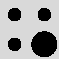
\includegraphics{tex-images/hop_toi_4_hat_3_bk_1_va_1_bk_2/hop_toi_4_hat_3_bk_1_va_1_bk_2.pdf}
    \caption{Hộp tối chứa bốn hạt, ba hạt bán kính 1 và một hạt bán kính 2.}
    \label{fig:hop_toi_4_hat_3_bk_1_va_1_bk_2}
\end{figure}
\begin{figure}[h!]
    \centering
    
\includegraphics{tex-images/hop_toi_4_hat_2_trang_bk_1_va_1_den__bk_1_va_1_den_bk_2/hop_toi_4_hat_2_trang_bk_1_va_1_den__bk_1_va_1_den_bk_2.pdf}
    \caption{Hộp tối chứa bốn hạt, hai hạt trắng bán kính 1, một hạt đen bán kính 1 và 1 hạt đen bán kính 2.}
    \label{fig:hop_toi_4_hat_2_trang_bk_1_va_1_den__bk_1_va_1_den_bk_2}
\end{figure}

Với hộp tối, bạn sẽ có một công cụ linh hoạt để tư duy và nghiên cứu, từ các tình huống đơn giản đến những mô hình ngẫu nhiên phức tạp trong thế giới xác suất và thống kê.
\end{document}
